\chapter{Traitement de Langage Naturel (TLN)}
\section{Introduction}
Le Traitement de Langage Naturel (Natural Langage Processing) est une approche pour analyser des textes qui est basé sur les théories et la technologies. C'est un domaine très répandu actuellement dans la recherche et développement \citep{natural-language-processing}. La NLP est utilisé dans la \emph{recherche d'information}, \emph{traduction des textes}, \emph{traduction des voix}, \emph{système de question réponse} ainsi que diverses domaines. Citons quelques définitions parmi tant d'autres.

\begin{definition}
    Le Traitement de Langage Naturel (TLN) est un discipline qui combine la linguistique, l'informatique et l'intelligence artificielle pour analyser et étudier les interactions entre uns système informatique et une langage naturel humain. La Recherche d'Information est parmi l'une de tâche du NLP \citep{art-nlp}.
\end{definition}

\begin{definition}
    Selon \citeauthor{natural-language-processing}, le TLN est un ensemble des techniques informatiques théoriques, pour analyser et représenter naturellement des textes (dans un langage quelconque) en passant par un ou plusieurs niveaux d'analyse linguistique dans le but de parvenir a traiter le langage humain dans une tâche ou applications \citep{natural-language-processing}.
\end{definition}

L'analyse de langage, porte a connaître la structure de langage tel que les mots, les significations, combinaison des mots, ainsi que la contribution des mots au sens de la phrase. Et aussi d'analyser le fonctionnement du monde et le raisonnement de l'humanité dans le monde \citep{automatic-nlp}.

Le domaine du TLN comporte des divisions tel que:
\begin{itemize}
    \item \textbf{Traitement de Langage Naturel (NLP)}: production de représentation significatif. Équivalent du rôle de lecteur et écouteur.
    \item \textbf{Génération de Langage Naturel (NLG)}: production de langage a partir d'une représentation. Équivalent du rôle d'auteur et interlocuteur.
    \item \textbf{Compréhension de langage (Language Understanding)}: Termine avec un langage orale.
    \item \textbf{Compréhension de langage orale (Speech Understanding)}: Démarre avec un langage orale. Permet de savoir comment un langage orale va se traduire en texte.
\end{itemize}

Le domaine de TLN par rapport a l'intelligence artificielle est illustré dans la Figure~\ref{fig:nlp-ref-ai}.

\begin{figure}[htbp]
    \begin{center}
        \fbox{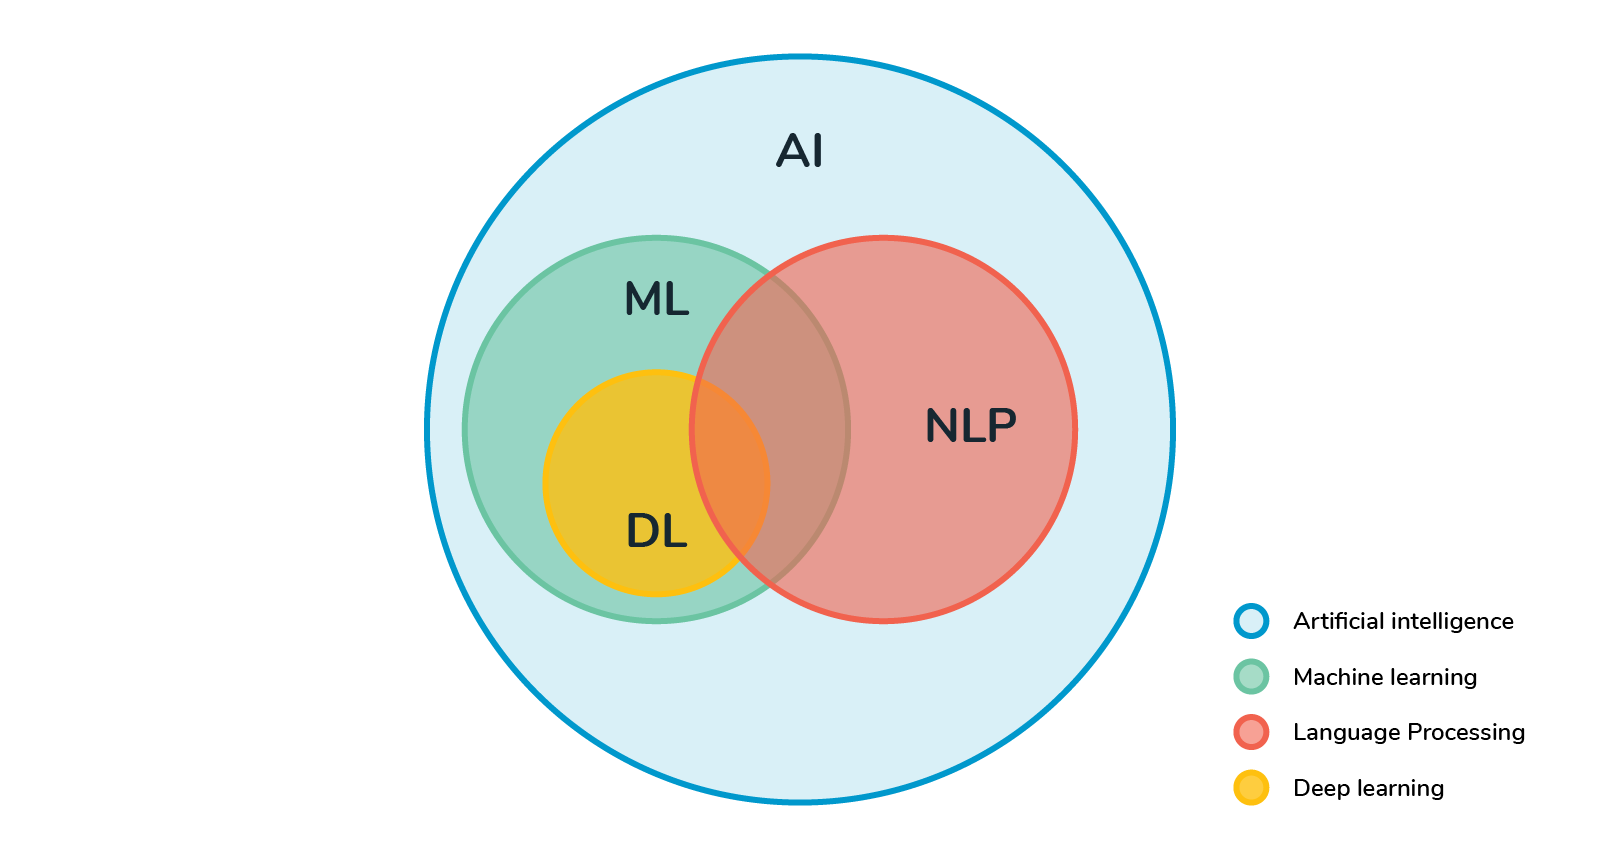
\includegraphics[width=13cm, angle=0]{Figures/NLP/nlp-ref-ai.png}}
    \end{center}
    \caption{Intelligence Artificiel et Traitement de Langage Naturel \citep{devopedia-nlp}}\label{fig:nlp-ref-ai}
\end{figure}

Certains notion qu'on abordera ici sont déjà présenté dans la Section~\ref{sec:processus-ri}, et qui ne seront pas détaillés.

\section{Un peu d'histoire}
Cette brève histoire est tiré de l'ouvrage de \citeauthor{natural-language-processing} \citep{natural-language-processing}. La recherche en Traitement de Langage Naturel trouve ses origines dans les années 1940. Le \emph{MT (Machine Translation)} est la première application en TLN qui est une application d'ordinateur. En 1946, Weaver et Booth démarre l'une de projet récent de MT, encore sur la traduction basé sur l'expertise de voler le code d’ennemie durant la deuxième guerre mondiale. Ce projet a suggérer l'utilisation de la cryptographie et de la théorie de l'information pour le traduction de langage. Puis la recherche sont devenu varié dans les institutions en États-Unis d'Amérique (USA).

En 1957, Chomsky a publié \textit{Syntactic Structure}, qui introduit l'idée de grammaire générative pour remédier aux problèmes rencontré dans les années antérieurs tel que l’ambiguïté syntaxique, \dots Une autre domaine de TLN commence aussi a émerger, comme la reconnaissance vocale.

La communauté de \emph{traitement de langage} et la \emph{communauté vocale} (Speech community) étions divisé alors en deux camps: d'une part la communauté de traitement de langage dominé par la théorie perspective de grammaire germinative et hostile en méthode statistique; et d'autre part la communauté vocal (Speech Community) dominé par la théorie statistique de l'information et hostile en théorie linguistique.

En 1950, l'homme pense que la meilleur qualité totalement automatique peut produire des résultats indiscernable de la translation humaine, et qu'un tel système peut être opérationnel dans quelques années.

Enfin, le TLN a connu beaucoup d'évolution ainsi des nombreuses lacunes. A partir des années 1980, le TLN a évolué beaucoup plus vite par la dispositions des ressources computationnel ainsi que des ordinateurs performants.

\section{Les niveaux de langage}
Un langage comporte généralement cinq niveaux ou étape de traitement \citep*{automatic-nlp, handbook-nlp}, illustré dans la Figure~\ref{fig:nlp-stage}:
\begin{itemize}
    \item \textbf{Phonétique et phonologie}: analyse la liaison des mots et des phrases au son qui les réalisent a l'oral. Cette niveau n'est pas utile dans le traitement de langage textuelle.
    \item \textbf{Morphologie}: analyse la façon dont les mots sont construits, et de connaître leurs rôles dans la phrase.
    \item \textbf{Syntaxe}: analyse la façon dont les mots se combinent pour former des \textit{syntagmes}, puis des proposition et enfin des phrases correctes. Un \textbf{syntagmes} est un unité syntaxique intermédiaire entre le mot et la phrase, et comprenant un seul noyau et souvent des compléments.
    \item \textbf{Sémantique}: analyse la façon dont les mots font du sens lorsqu'ils sont insérés dans une phrase indépendamment du contexte.
    \item \textbf{Pragmatique}: analyse la façon d’interpréter les phrases selon leur contexte d'énonciation comme l'interlocuteur, phrase précédente, connaissance commune du monde, \dots
\end{itemize}

\begin{figure}[htbp]
    \begin{center}
        \fbox{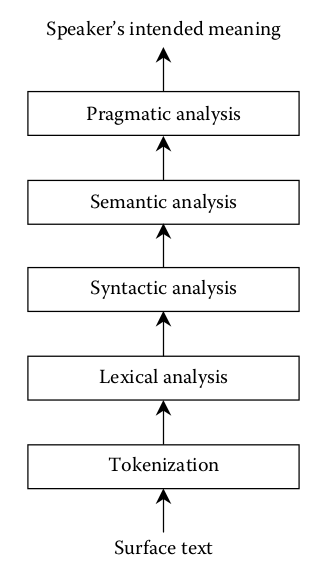
\includegraphics[width=8cm, angle=0]{Figures/NLP/nlp-stage.png}}
    \end{center}
    \caption{Étape d'analyse de texte dans le TLN \citep{handbook-nlp}}\label{fig:nlp-stage}
\end{figure}

\section{Phonologie}
La phonologie interprète le langage parlé (son de parole) dans un mot \citep{natural-language-processing}. Il y a trois règles tel que:
\begin{itemize}
    \item \textbf{Règle phonétique}: pour les sons dans les mots.
    \item \textbf{Règle phonémique}: pour les variations de prononciation quand les mots son prononcé ensemble.
    \item \textbf{Règle prosodique}: pour la variation d'un stresse et d'intonation dans un phrase.
\end{itemize}

\section{Morphologie}
La morphologie est l'étude de la forme des mots tel que leur \textit{flexion}: indication de cas, genre, nombre, mode et temps; leur \textit{dérivation}: préfixes, suffixes et infixes; leur \textit{composition}: mots composés. C'est aussi une analyse morphosyntaxique, qui analyse des règles de combinaison des morphèmes selon la configuration syntaxique de l’énoncé. La morphologie consiste a segmenter des textes en unités élémentaire qu'on appelle \textit{tokenisation} et à déterminer les différentes caractéristiques de ces unités \citep{automatic-nlp,natural-language-processing}.

Un humain est capable de faire ce traitement pour comprendre le sens, vu que chaque sens des morphèmes ne change pas dans tous les mots, et même pour un système TLN qui consiste a reconnaître le sens porté par chaque morphème pour représenter le sens \citep{natural-language-processing}.

\begin{definition}[Lemme]
    On appelle \textit{lemme} la racine d’un mot, sans ses marques d’accord, de conjugaison, de cas. L'entrée d'un dictionnaire est généralement un lemme. Le lemme est nécessaire dans toute analyse sémantique. \citep{automatic-nlp}
\end{definition}

\begin{definition}[Flexion]
    Les \textit{flexions} sont les modifications opérées sur le lemme pour distinguer les formes de conjugaison (personne, temps, mode, voix – flexion verbale) ou le genre, le nombre et le cas (flexion nominale). L’opération qui consiste à retrouver ces informations est la \textit{lemmatisation}, ou souvent appelé \textit{racinisation (stemming)} \citep{automatic-nlp}.
\end{definition}

\begin{definition}[Morphème]
    On appelle \textit{morphème} le plus petit unité ou unité minimale de sens \citep{natural-language-processing}. Par exemple, le mot prétraitement est composé de trois morphèmes tel que le préfixe \textbf{pre}, la racine \textbf{traite} et la suffixe \textbf{ment}.
\end{definition}

Cette étape est une partie essentiel du TLN, qui est nécessaire pour définir les caractères, mots et phrases dans un document. Elle relève un défi tel que la \emph{résolution des ambiguïtés} dans le langage naturel ainsi que de convertir des fichiers textes dans un séquence de texte bien défini avec un sens. Cette étape peut être divisé en deux parties: \textit{Triage de document (Document Triage)} et \textit{Segmentation de texte (Text Segmentation)} \citep{handbook-nlp}.

\subsection{Triage de document}
Le triage de document c'est l'action de convertir un ensemble des fichiers en documents textuelles bien définie. Il se décompose en trois étapes tel que:
\begin{enumerate}
    \item \textbf{Identification d'encodage de caractère (Character Encoding Identificator)}: permet d'identifier l'encodage de caractère utilisé dans le fichier a convertir, par exemple si le fichier utilise l'encodage UTF-8, etc.
    \item \textbf{Identification de langage (Language Identification)}: permet de déterminer dans quelle langue le fichier est écrit (Français, Anglais, etc.).
    \item \textbf{Sectionnement de texte (Text Sectionning)}: permet d'identifier le contenu textuel du fichier pour pouvoir le convertir en document textuel bien défini.
\end{enumerate}

\subsection{Segmentation de texte}
La segmentation de texte est un étape cruciale et complexe dans le Traitement de Langage Naturel. Il consiste a convertir un document textuel bien définie en composant des mots et des phrases \citep{handbook-nlp}. C'est aussi la transformation d'un alignement d'un caractère en une unité élémentaire souvent des mots et phrase \citep{automatic-nlp}. Généralement, il y a trois étapes tel que la \textit{segmentation de mot (Word segmentation)}, la \textit{normalisation de texte (Text Normalization)} et la \textit{segmentation de phrase (Sentence Segmentation)}.

Pour la segmentation de texte, il faut définir une liste de caractères délimiteur pour pouvoir segmenter le texte (espace, ponctuation, apostrophe). Pour les langages dont l'espace n'est pas un délimiteur comme la langue chinoise par exemple, cette segmentation est plus complexe \citep{handbook-nlp}. Et même avec la langue qui a comme délimiteur les trois caractères cités ci-dessus, il est quand même difficile de séparé les mots, car l'apostrophe peut être utilisé dans un seul mot comme \textit{aujourd'hui}, aussi un unité élémentaire peut contenir des espaces comme \textit{pomme de terre} \citep{automatic-nlp}.

En pratique le système de segmentation du texte utilise une liste de séparateurs par défaut, a laquelle ils ajoutent des connaissances lexicales et morphosyntaxiques pour traiter les cas ambigus. Chaque lange possède ses propres connaissances lexicales.

\subsubsection*{Segmentation de mot}
La segmentation de mot c'est l'action couper un séquence des caractères en texte par la localisation de délimiteur de mot (\emph{Word boundaries}) pour pouvoir être utilisé dans la traitement linguistique. Un délimiteur permet de définir le point où un mot est terminé et qu'un autre commence. Les mots obtenues sont appelées des \textit{tokens}, et la façon d'obtenir ces tokens est la \textit{tokenisation} ou \emph{tokenization} en anglais \citep{handbook-nlp}.

Pour les langages délimité par un espace (\emph{space-delimited}), souvent des langages européennes, les mots sont séparés par des espaces. Tandis que pour des langages qui ne sont pas délimités par un espace comme le Chinois et le Thaï, il n'y a pas d'indication sur le délimiteur \citep{handbook-nlp}. Dans le cadre de ce devoir, on travaillera sur des langages délimité par un espace.

Dans un langage délimité par un espace, les ponctuations sont souvent traité comme des tokens séparés, mais qui varie d'un langage a un autre. Mais pose souvent des problèmes comme des abréviation, les quottes et les apostrophes. \citep{handbook-nlp}

\subsubsection*{Normalisation de texte}
La normalisation de texte permet de fusionner les différentes formes de token en une forme canonique normalisé par exemple Mr et Monsieur. Cette normalisation permet aussi de normaliser des dates, des heures, des formats monétaires et d'autre informations numériques. Par exemple, les trois tokens écrit \$300 peut être prononcé comme \og{trois cent dollars} \fg{} et la normalisation de texte peut convertir le token original en token désiré. \citep{handbook-nlp}

\subsubsection*{Segmentation de phrase}
C'est de déterminer comment le texte doit être divisé en phrase pour un traitement plus avancé. En identifiant les délimiteurs de phrase (souvent un point pour la langue délimité par un espace). Souvent la segmentation de phrase est référencé comme \textit{détection de délimiteur de phrase} ou \textit{désambiguïsation de délimiteur de phrase} ou encore \textit{reconnaissance de délimiteur de phrase} \citep{handbook-nlp}.

\subsection{Catégories grammaticales}
Les catégories grammaticales est une information morphosyntaxique importante. Ces catégories sont souvent des noms, verbe, adjectif, mais qui varie selon le système. Par exemple \textit{Penn Treebank} contient 45 catégories. Sur la Figure~\ref{fig:categorie-grammaticale} un exemple de catégorie grammaticale pour la phrase \textit{\og~Qui veut noyer son chien l’accuse de la rage~\fg{}}, et qui illustre aussi la problème d’ambiguïté pour cette phrase. En général 25\% du lexique est de forme ambigus pour la langue française. Et un exemple de description morphosyntaxique illustré dans la Figure~\ref{fig:exemple-desc-morphosyntaxique}.

\begin{figure}[htbp]
    \begin{center}
        \fbox{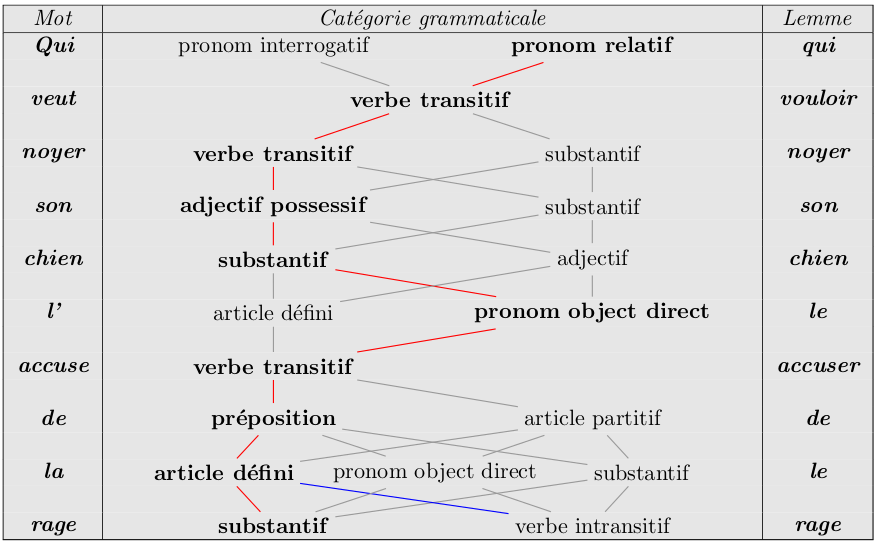
\includegraphics[width=15cm, angle=0]{Figures/NLP/classe-grammatical.png}}
    \end{center}
    \caption{Catégorie grammaticale \citep{handbook-nlp}}\label{fig:categorie-grammaticale}
\end{figure}

\begin{figure}[htbp]
    \begin{center}
        \fbox{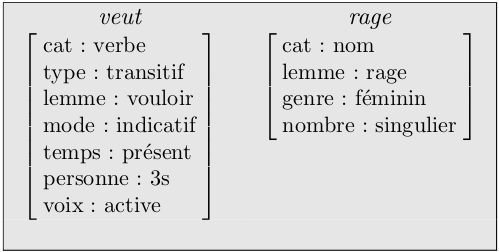
\includegraphics[width=10cm, angle=0]{Figures/NLP/description-morphosyntaxique.png}}
    \end{center}
    \caption{Description morphosyntaxique \citep{handbook-nlp}}\label{fig:exemple-desc-morphosyntaxique}
\end{figure}

\section{Analyse lexicale}
Un humain ou un Système TLN interprète le sens de chaque mot individuellement. L'analyse lexicale permet alors de déterminer le sens de chaque mot individuellement. Le but est de contribuer au compréhension de niveau de mot par une affectation de tag \textit{part-of-speech} pour chaque mot. Un mot qui a un sens possible peut être remplacé par un représentation sémantique de ce sens \citep{natural-language-processing}.

Un analyse lexicale utilise un connexion, qui est déterminé et choisi par le système TLN\@. Un lexicon peut être \textbf{simple} c'est à dire des mots et ses \textit{pos (part of speech)} ou peut être \textbf{complexe} et contient l'information de classe sémantique des mots \citep{natural-language-processing}.

\section{Syntaxe}
La syntaxe décrit comment les lemmes ou flexions sont ordonnées pour créer des constituants, composant aux-mêmes des phrases. Souvent, l'analyse syntaxique est représenté de façon hiérarchique. Dans l'analyse syntaxique, on travaille avec les mots, les phrases, ainsi que l'étape de la formation du mots a la phrase \citep{automatic-nlp}. L'analyse syntaxique est une analyse complexe avec différentes niveaux, les détails ne seront pas traité dans ce devoir, mais présent dans \citetitle[section 3]{automatic-nlp} \citep{automatic-nlp}.

L'analyse syntaxique selon \citeauthor{natural-language-processing}, se focalise sur l'analyse des mots dans une phrase, pour découvrir la structure grammaticale de la phrase, qui nécessite l'utilisation de la grammaire et un parseur. Dans l’analyse syntaxique, l'ordre et le dépendance des mots contribue au sens: par exemple, la phrase \textit{\og~Le chat attaque le chien~\fg{}} et la phrase \textit{\og~Le chien attaque le chat~\fg{}} ont un sens différent car ses termes de syntaxe sont différents, pourtant ils sont composé des mêmes mots \citep{natural-language-processing}.

\subsection{Analyse superficielle}
Le but de l'analyse superficielle ou partielle \citep{automatic-nlp}, est de reconnaître les syntagmes simples, non récursif d'un énoncé sans lier les uns aux autres; d'obtenir des résultats moins riches mais plus sûr et plus rapide. Cette approche s'oppose a l'analyse profonde ou complète qui cherche a regrouper chaque phrase dans une unique représentation.

\textbf{Cass} est un exemple de d'analyseur partielle efficace, qui consiste en une cascade d'automates à états finis.

\subsection{Analyse en dépendance}
L’analyse syntaxique en dépendance diffère surtout de l’analyse en constituants (comme les règles hors-contexte) par le mode de représentation. Les deux approches n’ont pas de différence au niveau de leur couverture ou de leur expressivité (A reformuler). L'idée est de relier les mots et non les constituants \citep{automatic-nlp}.

Un exemple de grammaire de dépendance est la \emph{Link Grammar} qui définit la lexique et les contraintes d'attachement, comme illustré dans la Figure~\ref{fig:link-grammar} et la Figure~\ref{fig:link-grammar-syntax}

\begin{figure}[htbp]
    \begin{center}
        \fbox{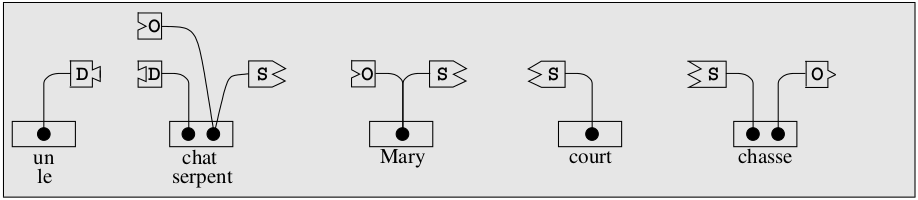
\includegraphics[width=13cm, angle=0]{Figures/NLP/lexic-link-grammar.png}}
    \end{center}
    \caption{Exemple de définition de la lexique \emph{Link Grammar} \citep{automatic-nlp}}\label{fig:link-grammar}
\end{figure}

\begin{figure}[htbp]
    \begin{center}
        \fbox{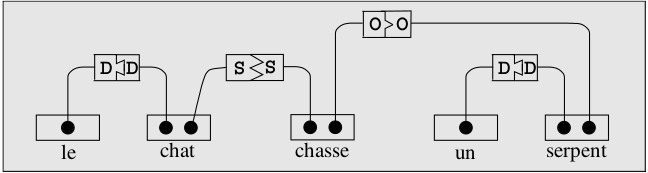
\includegraphics[width=13cm, angle=0]{Figures/NLP/syntax-link-grammar.png}}
    \end{center}
    \caption{Exemple d'analyse syntaxique avec \emph{Link Grammar} \citep{automatic-nlp}}\label{fig:link-grammar-syntax}
\end{figure}

\section{Sémantique}
Un approche sémantique peut être utilisé pour réduire les ambiguïtés syntaxiques, a mieux cibler des contextes (en RI par exemple), mais son but finale est de représenter formellement l’information véhiculée par un énoncé et éventuellement d’en inférer des nouvelles connaissances ou une réponse à la question posée dans le cas où l'énoncé est une question \citep{automatic-nlp}. Il a pour but d'associer a un séquence de mots une représentation interne de son sens, tout en prenant compte l'utilisation futures des résultats obtenues.

Selon beaucoup des personnes, c'est dans le niveau sémantique qu'on détermine la signification, pourtant tous les niveaux contribuent au signification. La sémantique détermine alors la signification possible d'une phrase en se concentrant sur l'interaction parmi les significations de niveau des mots dans une phrase, avec la possibilité de désambiguïsation sémantique des mots aux multiple sens. Par exemple si on prend le mot \textbf{pile}, ça peut être un pile pour alimenter un appareil électronique, ou ça peut être un structure dans un langage de programmation informatique.

Selon \citeauthor{automatic-nlp}, il y a quatre méthodes:
\begin{itemize}
    \item \textbf{L'analyse profonde}: permet d'obtenir une représentation complète de l’énoncé
    \item \textbf{Interprétation sémantique grammaticales}: qui s'appuie sur une analyse syntaxique totale
    \item \textbf{Grammaires sémantiques}: qui modélisent les données spécifiques
    \item \textbf{Patrons sémantique}: qui détectent les informations prédéfinies dans un texte
\end{itemize}

On distingue deux types de sémantique tel que la \textit{sémantique grammaticale} qui se charge a construire un sens de l'énoncé globale, et la \textit{sémantique lexical} qui étudie la participation des mots a ce sens et tous les ambiguïtés qu'ils provoquent.

\citeauthor{amelioration-ri-approche-semantique,approche-semantique} \citep{amelioration-ri-approche-semantique,approche-semantique} ont chacun développé un moteur de recherche basé sur cette notion de sémantique pour améliorer la qualité de recherche, et analyser les ambiguïtés dans un terme de recherche des utilisateurs.

\subsection*{Quelques relations importantes entre les mots}
Citons les relations importantes entre les mots \citep{automatic-nlp} qui sont nécessaire en analyse sémantique tel que:
\begin{itemize}
    \item \textbf{Polysémie et l'homonymie}: propriété de certains formes graphiques (signifiants) de renvoyer à plusieurs sens (signifié). Par exemple, le mot \textit{bureau}.
    \item \textbf{Synonymie}: lien entre deux mots ayant la même sens.
    \item \textbf{Hyponymie}: relation d'inclusion entre deux mots dont l'un (hyponymie) est plus spécifique que l'autre (hyperonyme). Par exemple le mot \textit{gorille} est un hyponymie du mot \textit{quadrumane}, le mot \textit{fleur} est un hyperonymie du mot \textit{tulipe}.
    \item \textbf{Méronymie et holonymie}: relation de partie a tout. Par exemple, une serrure est une partie d'une cage (méronymie), un bâtiment contient une pièce (holonymie).
\end{itemize}

Ces relations existant entre les mots sont répertoriés dans des base informatiques dont le plus utilisés est \textbf{WORDNet}.

\section{Pragmatique}
\citeauthor{natural-language-processing} cite un niveau supplémentaire entre la sémantique et la pragmatique, c'est le \textbf{discours} qui travaille sur un texte plus longue qu'une phrase et interprète le sens en connectant tous les phrases. Il y a deux types de traitement de discours tel que: l'\textit{Anaphore} et le \textit{Discours/text structure recognition}.

Tandis que l'analyse pragmatique sert dans un situation bien spécifique, utilise de contexte qui dépasse le contenu de compréhension de texte \citep{natural-language-processing}. En d'autres termes, il regroupe un grand nombre de domaine qui englobent tous les problèmes qui ne pouvant être traités avec la syntaxe et la sémantique \citep{automatic-nlp}. Cette analyse nécessite l'utilisation des connaissances extra-linguistiques sur le contexte et du discours. Pour cette raison que les application pratiques sont rares, pourtant il y a quelques uns \citep{automatic-nlp} comme la \textit{déictique}, l'\textit{implicatures conversationnelle} et la \textit{présupposition}.

\section{Approche du TLN}
Il y a généralement trois approche dans la Traitement de Langage Naturel, tel que l'\textit{approche symbolique}, l'\textit{approche statistique} et l'\textit{approche connexionniste}.

\subsection{Approche symbolique}
Cette approche a coexisté avec l'approche statistique le jour après la naissance de ce domaine. Elle fait une analyse profonde des phénomènes linguistiques, et qui est basé sur la représentation explicite des faits a propos d'un langage a travers une connaissance bien compris. Cette approche a été trouvé dans un système basé sur des règles (ensemble des règles, moteur d'inférence et un espace de travail); ou logique: structure sans forme de proposition logique.

L'approche symbolique est appliqué dans diverses domaines de recherche comme l'\textit{extraction d'information}, la \textit{catégorisation de texte}, \textit{résolution d’ambiguïté}, et l'\textit{acquisition lexicale}.

\subsection{Approche statistique}
Cette approche, souvent utilisé un large volume de texte (corpora), emploi des techniques mathématiques variés pour développer des modèles approximatif généralisé de phénomène linguistique. Cette approche utilise des données observables comme source primaire d'évidence. Le modèle statistique souvent utilisé est le \emph{HMM} ou \emph{Hidden Markov Model}.

L'approche statistique est appliqué dans la \textit{reconnaissance vocale}, \textit{acquisition lexicale}, \textit{parsing}, \textit{part-of-speech tagging}, \textit{machine de translation statistique}, \textit{collocations}, \textit{apprentissage statistique de grammaire}.

\subsection{Approche connexionniste}
Cette approche est apparu dans les années 1960, est comme l'approche statistique qui développe des modèles généralisés depuis l'exemple de phénomène linguistique. Elle combine l'apprentissage statistique avec différentes \emph{théories de représentation} qui permet la transformation, l'inférence et la manipulation de formule logique.

Certains modèles de l'approche connexionniste s'appelle \textbf{modèle localiste} qui peut faire des tâches comme \emph{désambiguïsation de sens de mot}, \emph{génération de langage}, et \emph{inférence limité}; et \textbf{modèle distribué} qui est utilisé pour les tâches comme la \emph{parseur des syntaxes (syntactic parsing)}, \emph{translation dans un domaine limité ou spécifique} et \emph{recherche associative}.

\section{Application de TLN}
La Traitement de Langage Naturel s'applique dans diverses domaines de recherche que ce soit textuelle ou sonores.

\subsection*{La Recherche d'Information (RI)}
Dans la recherche d'information, on travaille sur des textes, ce qui implique que certains implémentation utilise le NLP. Cette application utilise souvent l'approche statistique \citep{natural-language-processing}. Le TLN est généralement utilisé dans le niveau traitement morphologique.

Elle analyse la variation morphologique des mots ou \emph{stemming}, mais aussi la variation syntaxique (étude des syntagmes nominaux) ainsi que la variation sémantiques: relation liant des lemmes différents mais identiquement proches et la multitude de sens qui peut prendre une forme graphique donnée (polysémie, homonymie) \citep{automatic-nlp}.

\subsubsection*{Stemming}
\citep{automatic-nlp} La plus courante utilise une approximation des phénomènes linguistiques d'une langue donnée, comme les mécanismes habituels de conjugaison, d'accord ou de genre et en nombre, ou sa dérivation et tente de supprimer les suffixes tout en regroupant les différentes allomorphes (variante graphique d'une même racine).

L'algorithme le plus utilisé est celle de \emph{Lovins} et \emph{Porter} pour la langue anglaise et \emph{Jacques Savoy} pour la langue française.

\citep{stemming-algorithms} analyse de ces algorithmes, et les différentes approche sont illustré dans la Figure~\ref{fig:stemming-algorithms}.

\begin{figure}[htbp]
    \begin{center}
        \fbox{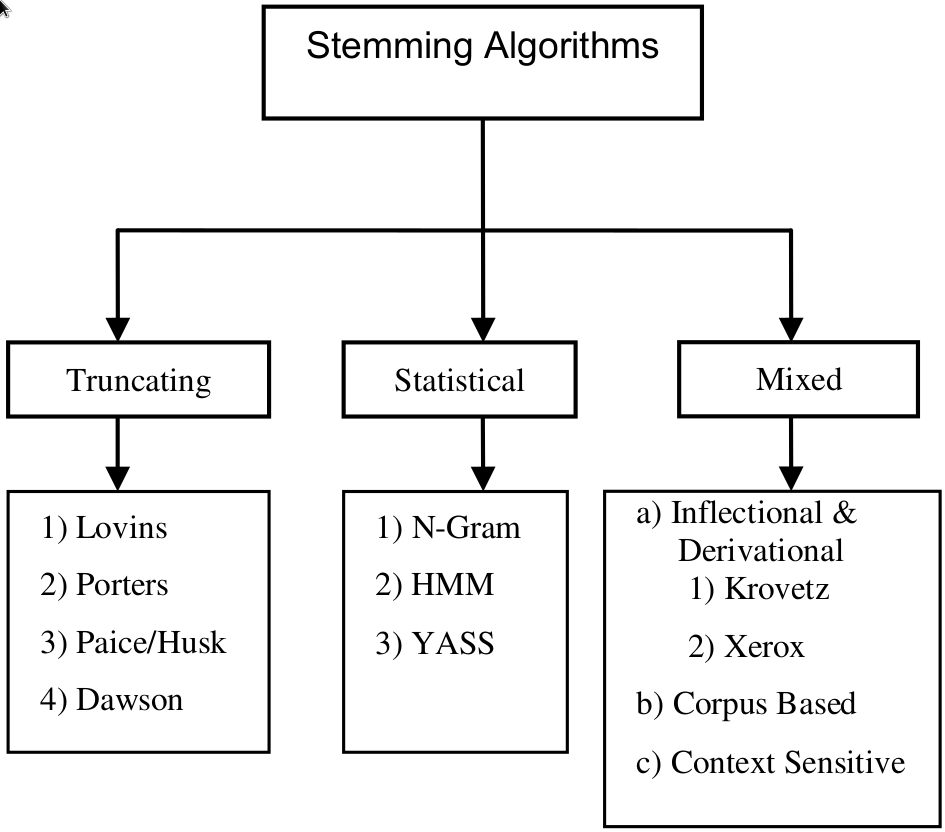
\includegraphics[width=13cm, angle=0]{Figures/NLP/stemming-algorithm.png}}
    \end{center}
    \caption{Algorithmes de stemming \citep{stemming-algorithms}}\label{fig:stemming-algorithms}
\end{figure}

\subsection*{L'Extraction d'Information (EI)}
Ce domaine d'application est plus récente, qui se base sur la reconnaissance, marquage (tagging), et extraction dans un représentation structurés, certains éléments clés d'information, par exemple: personne, compagnie, localisation, organisation, d'un large collection de texte \citep{automatic-nlp}.

\subsection*{Et d'autres applications}
Et d'autres domaines d'applications, comme la machine de traduction (Machine Translation), système de dialogue, système de question-réponse, système de résumé (summarization).

\section{Conclusion}
En conclusion, le Traitement de Langage Naturel est l'un de domaine intéressant, et contribue a beaucoup des recherches dans la domaine de l'informatique. Il est aussi nécessaire dans la recherche d'information. Elle se divise en deux principale branches qui est le traitement de langage écrite et le traitement de langage orale. Elle propose différentes approches et méthodes ainsi que différentes algorithmes pour faire des traitements. Elle est utilisés dans différentes domaines et qui est devenue indissociable de l'intelligence artificielle.